\section{Théorie}
\label{sec:theorie}
Lorsqu'un matériau est soumis à une contrainte telle qu'il ne rentre pas en mouvement, il est possible d'observer deux types principaux de déformation: élastique et plastique. Le cas étudié ici sera la déformation uniaxiale. Pour caractériser ces déformations il faut définir la contrainte $\ligma = F/S_0$ avec $F$ les forces uniaxiales appliquées et $S_0$ la surface de section de l'échantillon avant le début de la déformation. La contrainte produit la déformation $\varepsilon = \Delta l / l_0$ avec $\Delta l$ la variation de la longueur de l'échantillon dans l'axe des forces et $l_0$ cette longueur avant la déformation. Pour un essai de traction sur un échantillon métallique l'allure générale de la courbe de $\sigma(\varepsilon)$ est donnée en \autoref{fig:courbe_theorie}.
\begin{figure}[h]
    \centering
    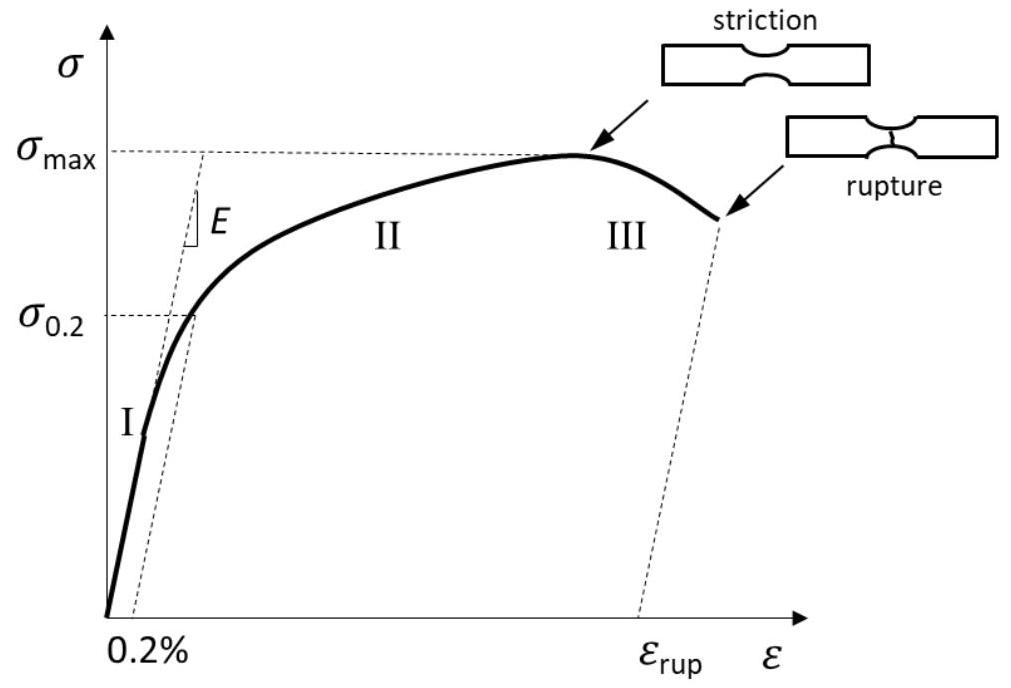
\includegraphics[width=0.6\linewidth]{figures/courbe_traction.png}
    \caption{Courbe de la contrainte $\sigma$ en fonction de la déformation $\varepsilon$ pour un métal générique dans un essai de traction \cite{notice}}
    \label{fig:courbe_theorie}
\end{figure}

Pour le cas de la déformation élastique, la zone $\mathbf{I}$ en \autoref{fig:courbe_theorie}, la relation entre contrainte et déformation est linéaire et donnée par:
\begin{equation}
    \ligma = E \varepsilon
\end{equation}
avec $E$ le module de Young du matériau. Cela correspond à la nature élastique des liaison atomiques qui s'agrandissent sous la contrainte. En l'appliquant, tous les atomes s'éloignent donc mutuellement mais de manière réversible, quand la contrainte diminue le matériau revient vers sa forme originale en suivant la même courbe de pente $E$.

Pour la déformation plastique il existe deux situations selon l'ampleur de la déformation. La première, correspondant à la zone $\mathbf{II}$ en \autoref{fig:courbe_theorie}, est le domaine plastique correspondant au début de la déformation irréversible. Si la contrainte est diminuée depuis ces niveaux de déformation le matériau suivra également une ligne de pente $E$ sur le graphique et arrivera à une déformation rémanente $\varepsilon_{\textrm{r}}$. C'est à l'aide d'une de ces déformations rémanentes que les domaines élastique et plastique sont arbitrairement délimités. Il est compliqué de mesurer expérimentalement la limite élastique d'un matériau comme étant le moment où la déformation n'est exactement plus réversible, cette limite est donc redéfinie avec le moment où la déformation rémanente vaut 0.2\% pour une contrainte $\ligma_{0.2}$. Lors d'un essai de traction il est donc possible de la mesurer en prenant une ligne de pente $E$ partant de la déformation rémanente de 0.2\% comme illustré en \autoref{fig:courbe_theorie}.

Lorsque la déformation est extrême le matériau subit une striction, à la zone $\mathbf{III}$ de la \autoref{fig:courbe_theorie}. Cela correspond empiriquement à une déformation plastique locale de l'échantillon qui amène si elle est poursuivie à la rupture. La déformation rémanente maximale est donc $\varepsilon_\mathrm{rup}$ obtenue en suivant la pente $E$ depuis le point de rupture comme illustré en \autoref{fig:courbe_theorie}.

Les déformations plastiques viennent d'un changement dans la structure du matériau ce qui est la raison de leur irréversibilité. Elles correspondent à une dislocation des atomes qui se déplacent dans le solide. Cela est illustré pour un type de dislocation, la dislocation "coin", en \autoref{fig:dislocation_slip}. 
\begin{figure}[h]
    \centering
    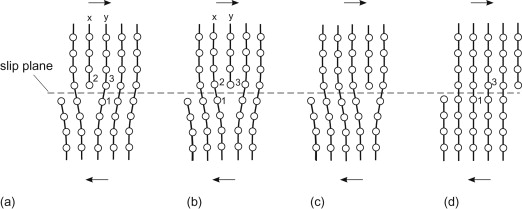
\includegraphics[width=0.8\linewidth]{figures/dislocations_slip.jpg}
    \caption{Illustration du mouvement d'une dislocation "coin" dans un cristal sous une contrainte \cite{manuel}}
    \label{fig:dislocation_slip}
\end{figure}
Ainsi des atomes se détachent et ce défaut se déplace de couches en couches du cristal. Il est cependant possible de limiter cet effet en introduisant de nouvelles espèces dans le solide. Ces nouveaux défauts peuvent venir bloquer le mouvement de ces dislocations s'ils sont présents sous la forme de précipités. Ces dislocations arrivent alors au niveau de ces défauts et y restent bloqués limitant la déformation plastique et rendant plus rigide le matériau. Il est donc possible dans un matériau de même composition d'avoir une plus ou moins grande ductilité selon la présence de précipités qui est elle même déterminée par le traitement thermique. En effet chauffer l'alliage à très hautes températures permettra de dissoudre les défauts dans le solide réduisant grandement la présence de précipités par exemple.
